\documentclass[12pt,letterpaper]{article}

%==================================================================================
% Template for the 13th International Association of Fire Safety Science (2019).  
%==================================================================================

% This template is based on the layout requirements of the Fire Safety Journal.  When submitting, please do include the *.tex and output (typeset) *.pdf files, figure files (photographs, diagrams, etc.), and any other ancillary files required to typeset your article.  The journal must be able to typeset your article with what you've provided.

% As with any programming language, there are multiple ways of executing any given task (e.g., figures, tables, maths, etc.).  The syntax in this template should be considered suggestions and not directives.  Please feel free to use your own favorite syntax, especially if it's more elegant than what is found below!  That said, the spacing and font parameters have been selected to conform to the appearance dictated by the journal (i.e. like MS Word).  Make sure your final typeset document has the correct formatting or it will be rejected.

% Required Packages ===============================================================
\usepackage{amsmath} % The usual maths package
\usepackage{amsfonts}  % The usual maths package
\usepackage{amssymb}  % The usual maths package
\usepackage[final]{graphicx} %Required for figures.
\usepackage{caption} % Needed to modify default figure captions
\usepackage{latexsym}
\usepackage{lineno} % Enables line numbers
\usepackage{parskip} % Makes a space between paragraphs like MS word
\usepackage{fullpage} % Overrides article margins
\usepackage{titlesec} % Enables modification of section labels
%\usepackage[numbib]{tocbibind} %Make References a numbered section
\usepackage{siunitx} % Formats the units and values
\usepackage{times}
\usepackage{chemformula}


%\usepackage{subcaption} % Enables multiple images in one figure environment
%\usepackage{xcolor} % For various font colors in figures
%===================================================================================

% The next two lines modify the font and font size of the section and subsection labels
\titleformat{\section}{\normalfont\bfseries}{\thesection}{0.2em.}{}
\titleformat{\subsection}{\normalfont\bfseries}{\thesubsection}{0.2em}{}

% This will change the figure captions from the default "Figure 1:" to "Figure 1."
\captionsetup[figure]{labelformat={default},labelsep=period,name={Figure}}

\linenumbers % Include line numbers throughout document

\begin{document} %====================================================================
\begin{flushleft} % Suppress the default full justification of text

% Title of your article
\textbf{Backdraft Experiments and Large Eddy Simulations in a Scaled Compartment}
\vspace{3mm}\\
%
% Author(s)
Marcos Vanella$^\text{a*}$, Ryan Falkenstein-Smith$^\text{a}$, and Thomas Cleary$^\text{a}$
\vspace{3mm}\\	

% Affiliation "b"
$^\text{a}$National Institute of Standards and Technology, Gaithersburg, USA  \\
marcos.vanella@nist.gov
\vspace{3mm}

$^*$Corresponding author

% Highlights/keywords ===================================================
\textbf{Highlights:}	
\begin{itemize}
	\itemsep-4pt % Override default vertical spacing among list items
	\item Initial conditions for computer fire models are defined from an extensive dataset of backdraft experiments performed at NIST.
    \item Chemical composition and heat measurements from these experiments are intended to assess fire models.
	\item The Fire Dynamics Simulator with fast chemistry is exercised on some of these backdraft scenarios.
	\item For mix-controlled fast reactions, ignition model temperature threshold and ignition procedure are found to play a primary role in backdraft outcomes. 
\end{itemize}
\vspace{3mm}

% Abstract ==============================================================	
\textbf{Abstract:}
%\vspace{3mm}
An extensive set of backdraft experiments has been performed at the NIST National Fire Research Laboratory. These experiments were conducted in a reduced scale compartment, and are part of defining the conditions conducive to backdraft. Further, the detailed chemistry and heat measurements are intended to evaluate computational fire models. In this article, we describe the modeling effort employing the Fire Dynamics Simulator (FDS) in simulations involving different fuels and ignition source locations mirroring a subset of the named experiments. We focus on using default simulation parameters and study their effect on the backdraft outcomes. In particular, the ignition model's temperature threshold and ignition procedure play a primary role in developing a backdraft.

\textbf{Keywords:}

Backdraft Experiments; Fire Simulation; FDS; Large Eddy Simulation; 

\section{Introduction}
Backdrafts pose a life-threatening risk to any firefighter that may encounter them. A backdraft is a deflagration resulting from igniting an incoming gravity current of air mixed with a heated, fuel-rich, and oxygen-depleted environment~\cite{fleischmann2013defining}. Several experimental works have identified the physical mechanisms and conditions conducive to backdrafts. Fleischmann examined the thermal and gas compositions within an enclosure's environment influencing the incoming gravity current~\cite{fleischmann1993backdraft,fleischmann1994quantitative}. Gottuk and others~\cite{gottuk1999development} estimated critical mass fractions in vitiated atmospheres, resulting in backdraft using full-scale steel compartments. Wu and colleagues~\cite{wu2011experimental} established a correlation between the likelihood of backdraft and compartment configuration by varying ventilation conditions, ignition locations, and mass fluxes of gas leakage. Other works have studied the probability of backdraft generated from solid fuel combustion within an enclosure~\cite{hayasaka2008backdraft,tsai2013full,zhao2021experimental}.

On the other hand, several studies have relied on computational models utilizing large eddy simulation (LES), particularly the Fire Dynamics Simulator (FDS), to simulate backdraft. In general, these studies use finite-rate chemistry and several-step reactions to capture deflagration physics. For example, Weng, Fan, and Hasemi used LES to predict the ignition time for backdraft in compartments with different opening geometries~\cite{weng2005prediction}. Ferraris and others implemented a subgrid-scale model based on mixture fraction to define partially premixed combustion applied to backdraft~\cite{ferraris2008large}. Park et al. used single and three-step finite rate chemistry in FDS to investigate the relationship between the initial fuel mass in a compartment and the resulting backdraft~\cite{park2017computational}.  Ashok and Echekki used FDS to study the effect of the gravity current magnitude on backdraft events~\cite{ashok2021numerical}. Of particular interest is the work of Myilsamy et al., who used single-step fast chemistry to study the fuel fraction required for backdraft in different opening geometries~\cite{myilsamy2019large}.
Several of these studies have established the critical elements that impact the generation of a backdraft. Yet, to date, a constraint has been the limited availability of comprehensive experimental datasets to compare simulation results. 

Recently, an extensive series of 500 experiments focused on examining backdraft in a reduced-scale enclosure was performed at the NIST National Fire Research Laboratory~\cite{Falkenstein2022}. The experimental series generated an extensive dataset that identifies environmental conditions indicative of backdraft under various configurations, including gaseous fuel type, fire size, spark location, and compartment opening configuration. The substantial range of comprehensive measurements provides detailed information that can be used to evaluate computational models. In this work, the wealth of experimental data produced is leveraged to assess the FDS default LES combustion models for backdraft, particularly two-step mixing controlled fast reactions in development for engineering applications.  

The next section describes experiments and their use in defining initial conditions within the compartment for backdraft simulation. Then, the standard FDS combustion model and the backdraft model setup are given in section~\ref{sec:FDS_setup}. A grid sensitivity study and comparison with experiments on representative backdraft cases using methane and propane is shown in section~\ref{sec:Grd_sens_exp}, and most importantly, effects of the re-ignition model and ignition procedure in deflagration outcomes are presented in sections~\ref{sec:ign_thr} and \ref{sec:ign_proc}. Finally, some conclusions are provided in section~\ref{sec:concl}.

%\textbf{Short description of the sections of the paper.}

\section{Experimental Method: Definition of compartment initial conditions}
\label{sec_exp_meth}

A schematic of the 1~m~by~1~m~by~1.5~m reduced-scale enclosure used for all experiments is provided in Figure~\ref{fig:Backdraft_experimental_setup}. The enclosure was designed to scale, 2/5\textsuperscript{th} the dimensions of an ASTM test room. Experiments were initiated when a square sand burner, with a 17.8~cm side length, was ignited. In these experiments, the sand burner's center was approximately 0.5~m from either side wall and 1.25~m from the front opening. After the initial ignition, the fire size increased to a predetermined heat release rate and was allowed to burn with the compartment door open for 60~s. Afterward, the door was shut. While the doorway was closed, fuel continued to flow through the burner for a predetermined duration, and when reached, the flow was stopped. The fuel flow durations used in this work are shown in Table~\ref{tab:Fuel_Flow_Time}, corresponding to their respective fire sizes. The compartment remained closed for an additional 30.0~s after the fuel flow duration to allow the internal gases to form a more homogenous mixture. Once the door opened, spark ignitors were triggered, providing a continuous ignition source for the residing fuel and incoming gravity current of air.
\begin{figure}[!]
	\centering
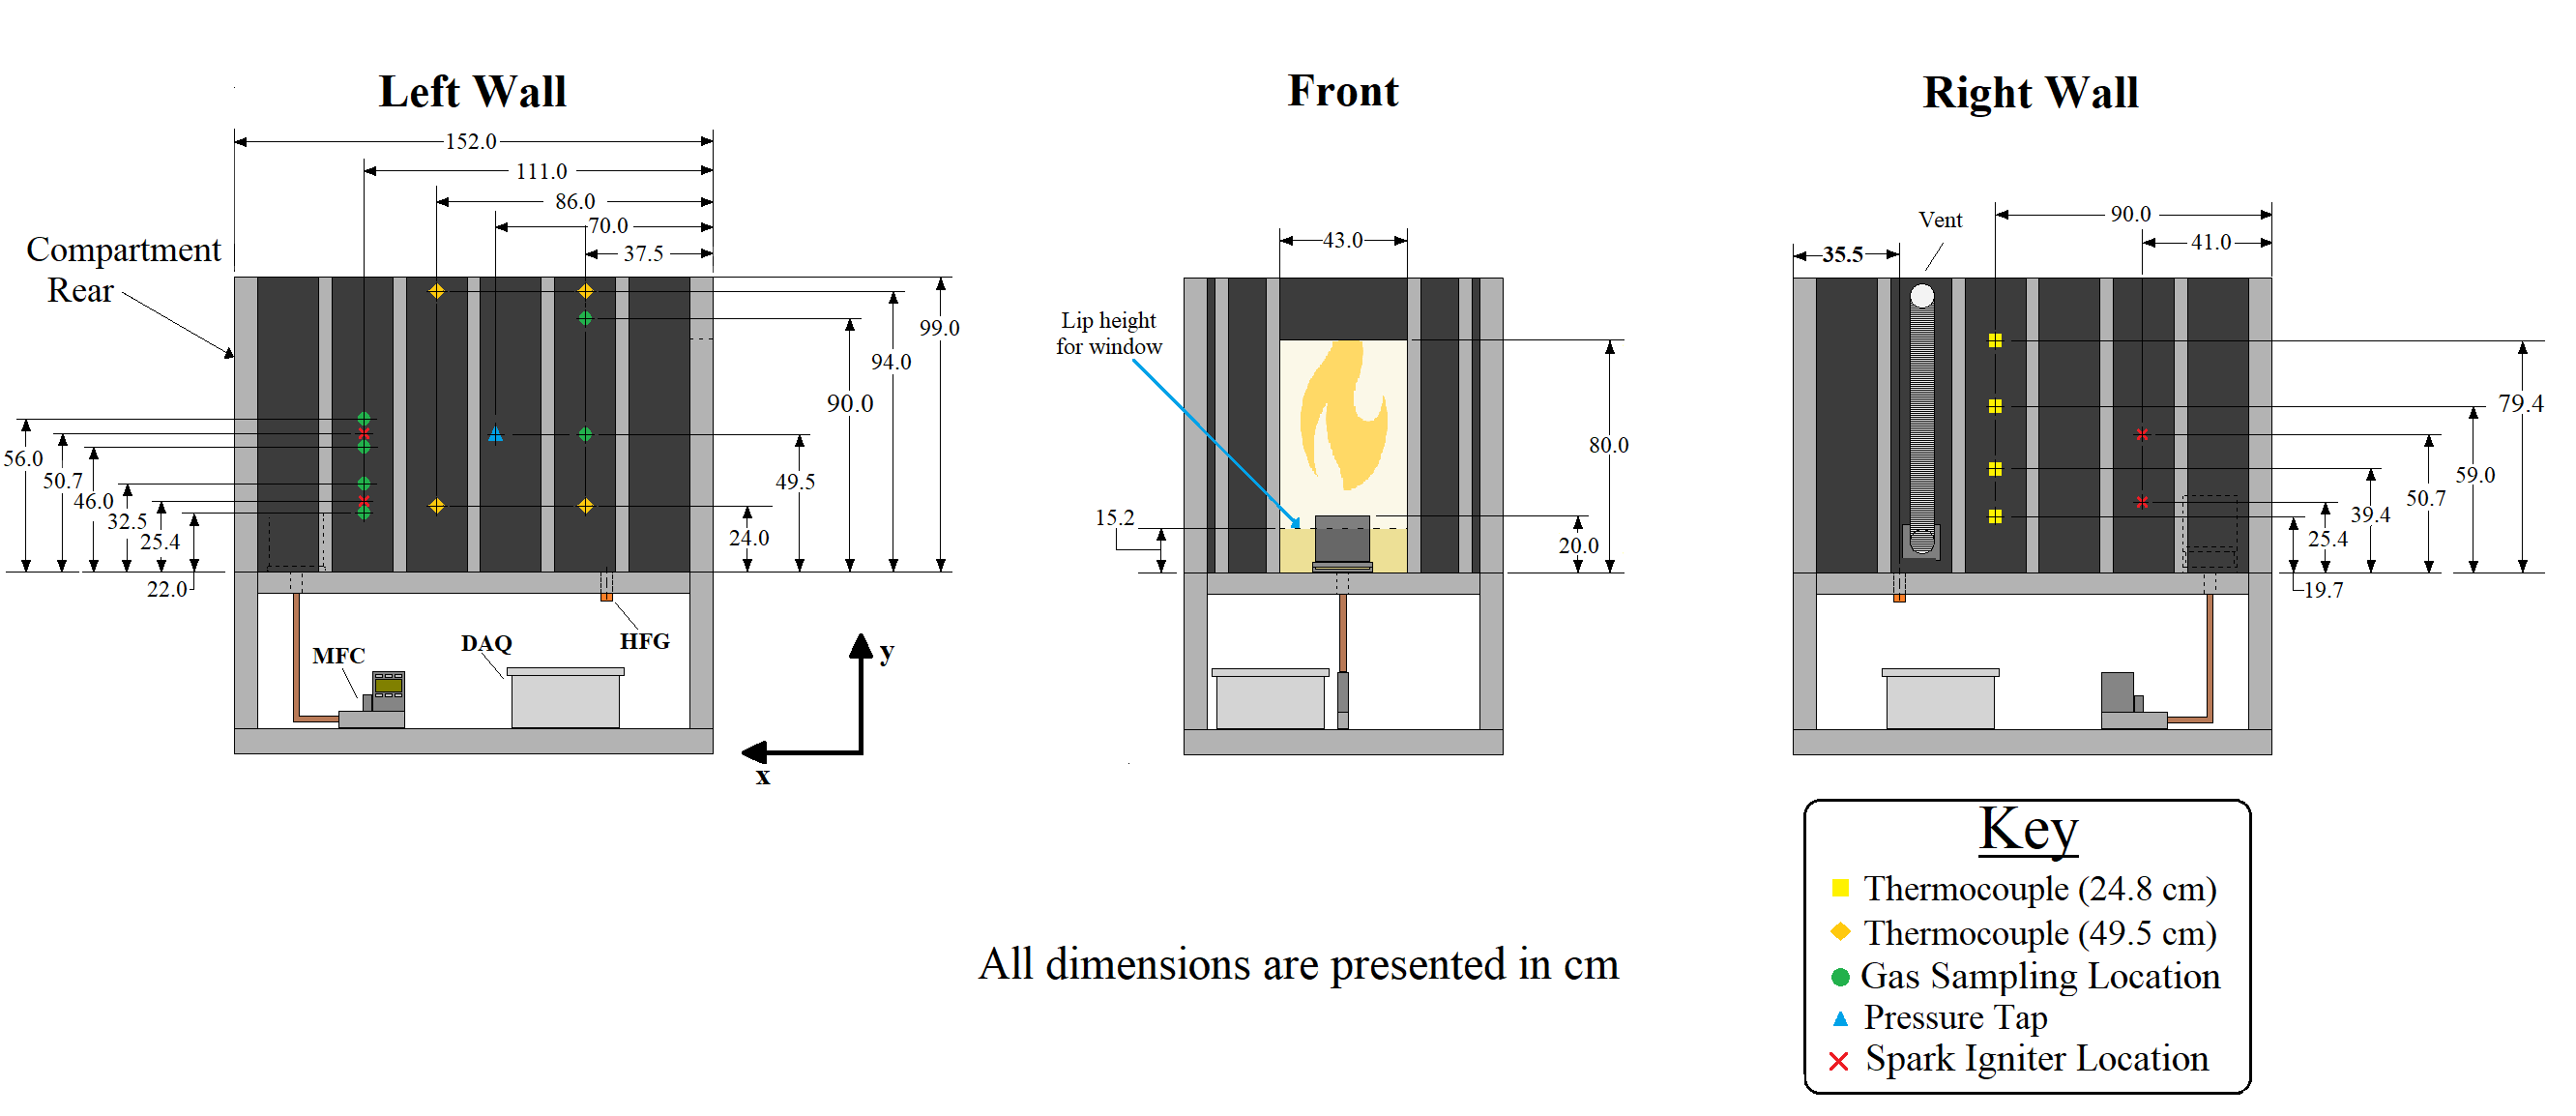
\includegraphics[width=16.0cm, keepaspectratio]{Experimental_Setup_6.png}
	\caption{Schematic of the $2/5^{\rm{th}}$ scale compartment used in backdraft experiments}
	\label{fig:Backdraft_experimental_setup}
\end{figure}

\begin{table}[h!]
\caption{List of fuel flow times for each fire configuration}
\label{tab:Fuel_Flow_Time}
\centering
	\footnotesize
	\begin{tabular}{c c l}
\hline
Fuel & Fire size~(kW)	& Fuel flow time~[FFT]~(s)  \\
\hline
Methane & 25.0~$\pm$~1.0~kW 	& 360,~390,~450\\
	& 37.5~$\pm$~1.0~kW 	& 225,~285      \\
%[0.075cm]
Propane & 16.7~$\pm$~1.0~kW		& 255,~270,~315	\\
	& 25.0~$\pm$~1.0~kW 	& 210,~285		 \\
\hline
\end{tabular}
\end{table}

The locations of the spark ignitors, thermocouples, and gas sampling locations are displayed in Figure~\ref{fig:Backdraft_experimental_setup}. The spark ignitors were positioned either 25.4~cm ('low spark') or 50.7~cm ('mid spark') from the compartment floor. Thermocouples were incorporated on both side walls of the compartment in two different configurations. The first thermocouple configuration used 49.5 cm long, 0.3175 cm diameter sheathed Type K thermocouples configured in a rectangular orientation on the left wall facing the door. The second thermocouple array included four 24.8 cm long, 0.3175 cm diameter sheathed Type K thermocouples configured in a line on the right wall facing the door spaced approximately 19.9 cm apart. Gas samples were portioned and analyzed into two gas analyzers and phi meters at one of three location pairs displayed in Figure~\ref{fig:Backdraft_experimental_setup}. The gas analyzer included one paramagnetic and two nondispersive infrared sensors to measure oxygen, carbon dioxide, and carbon monoxide, respectively. The phi meter~\cite{babrauskas1994phi,Falkenstein2021a} provided equivalence ratio measurements of the extracted gas sample. A combination of the gas analyzer and phi meter measurements was used to estimate the concentration of major species adjusted to a wet basis. Major gas species included methane/propane, oxygen, carbon dioxide, carbon monoxide, water vapor, and nitrogen. Gas and temperature measurements were monitored using a data acquisition system sampling 1.0~Hz during each experiment. Each experiment was recorded using two external cameras, with one placed nominally 5.5~m from the front and another approximately 4.7~m from the side of the compartment. A detailed description of the compartment is available in Ref.~\cite{Brown2022}.

Initial conditions for backdraft models were determined in two-compartment zones from time-averaged temperature and estimated gas concentration measurements averaged over repeated experiments with the same fuel flow duration and fire size. Zones were divided at the height of 39.25 cm from the species concentration measurements observed to be fairly homogeneous. Time-averaged measurements were calculated from a 10.0~s time domain immediately before the compartment doorway opening. 

An estimated gravity current velocity was computed using Eq.~\eqref{eq:vel_calc}, which utilizes a Froude number. The Froude number was determined from the ratio of the observed velocity of the gravity current, and the root of the product of the normalized positive density difference, $\beta$, the compartment height, $h$ (1.0~m), and the gravitational constant, $g$ (9.81~m s$^{-2}$). The observed velocity of the gravity current was estimated from the video recordings of the front of the compartment that captured the time to ignition from when the door opened. The density within the compartment before the door opened, $\rho$, and the density of the ambient fluid within the gravity current, $\rho_{o}$, estimated to be 1.19~g/L~$\pm$~0.01 from sensors outside of the compartment were used to calculate $\beta$. The gas mixture density within the compartment before the door opened was determined from the gas concentrations measured using the gas analyzer and phi meter. The average Froude number was determined to be 0.2~$\pm$~0.05. 
\begin{equation}
\label{eq:vel_calc}
U_{est}~\approx~\frac{1}{5}~{\sqrt{\beta~h~g}} \quad ; \quad \beta=\frac{\rho_{o}-\rho}{\rho}
\end{equation}

The uncertainty of the experimental measurements was determined from a combination of the Type A and B evaluation of uncertainty. The Type A evaluation of uncertainty was estimated from the variance of the averaged measurements. The Type B evaluation of uncertainty was determined from the reported instrumentation error. The variance between the averaged measurements was determined to be the dominant contributor to the estimated uncertainty.

Backdraft intensity was estimated from the total heat release of the exiting flame. During each experiment, the compartment was placed under a canopy hood with a 3.0~MW calorimetry measurement system. In this instance, the total heat release was estimated using carbon dioxide generation calorimetry with a correction for carbon monoxide generation to account for unburned fuel exiting the compartment. The total heat release, $THR$, was calculated using Eq.~\ref{eq:total_heat_release_corr}:
\begin{equation}
\begin{split}
\label{eq:total_heat_release_corr}
THR&=\sum_{t=0}^{\infty} \left[ \dot{m}_{\rm{CO_2}}(t)\left(\frac{\rm{LHV_F}~\rm{MW_F}}{\rm{x}~\rm{MW_{CO_2}}}\right)+\dot{m}_{\rm{CO}}(t)\left(\frac{\rm{LHV_F}~\rm{MW_F}}{\rm{x}~\rm{MW_{CO}}}-\Delta\rm{H}^{\rm{o}}_{C,CO}\right) \right] \Delta~t
\end{split}
\end{equation}
Here, $\dot{m}_{\rm{CO_2}}(t)$ and $\dot{m}_{\rm{CO}}(t)$ represent the mass flow rate of \ch{CO2} and \ch{CO} measured in the duct, respectively. The number of carbon atoms and lower heating value of the parent fuel are represented by $\rm{x}$ and $\rm{LHV_F}$, respectively. The molecular weight of the parent fuel, carbon dioxide, and carbon monoxide is denoted as $\rm{MW_F}$, $\rm{MW_{CO_2}}$, and $\rm{MW_{CO}}$, respectively. The heat of combustion for carbon monoxide, $\Delta \rm{H}^{\rm{o}}_{C,CO}$ used in Eq.~\ref{eq:total_heat_release_corr} was 10.10~kJ/g as reported by Ref.~\cite{Hurley2016}. The heat released from the combustion gases trapped in the compartment before opening the door is subtracted from the measured total heat released for a backdraft estimated from scores of experiments that did not ignite and produce a deflagration.

The probability of backdraft for different compartment configurations was determined from a regression fitting. The regression fitting incorporated the number of times a backdraft was observed over the total number of times the experiment was conducted under the same condition as a function of the total chemical energy within the compartment before an anticipated backdraft. Two different regression fittings for the likelihood of backdraft were calculated for different spark locations. 

\section{Numerical Method and Model setup} 
\label{sec:FDS_setup}

The Fire Dynamics Simulator (FDS) is a fire modeling software developed by the Fire Research Division of the National Institute of Standards and Technology, USA. It solves combusting, thermally buoyant flows with application to design and evaluation of fire protection systems, fire forensics studies, and general fire research, among others. Large eddy simulation based on eddy viscosity models, species transport, combustion, and radiation numerical models are at the core of this application. Of primary importance to the present work is the treatment of combustion in FDS, particularly the use of fast chemical reactions, which is essential to simulate realistic engineering problems in a cost-efficient manner. Fire generally involves non-premixed combustion, therefore, species mixing controlled reactions are treated using the Eddy Dissipation Concept (EDC) model~\cite{Magnussen:1}. Here, the volumetric mass of fuel consumed by the chemical combustion process is approximated as
%
\begin{equation}
  \dot{m}'''_f = - \rho \frac{\min({Y}_f,{Y}_{ox}/s)}{\tau_{mix}}
\end{equation}
where $\rho$ is the local cell density, ${Y}_f,{Y}_{ox}$ are the corresponding fuel and oxidizer mass fractions, $s$ is the stoichiometric ratio of the reaction, and $\tau_{mix}$ is the mixing process time scale that needs to be modeled~\cite{FDS_Tech_Guide}. From the volumetric mass consumption (or production) of the chemical species involved in the reaction, the heat release rate per unit volume, (HRRPUV)  can be computed as
%
\begin{equation}
  \dot{Q}''' = - \sum_j{\dot{m}'''_j \Delta h_{f,j}^\circ}
  \label{eq:HRRPUV}
\end{equation}
where $\dot{m}'''_j$ volumetric mass rate of change of species $j$, and $\Delta h_{f,j}^\circ$ is its enthalpy of formation. EDC and fast kinetics dispense with the need to integrate in-time reaction evolution equations on each computational cell, which generally becomes prohibitively costly for practical engineering problems. It also holds the unphysical assumption that any amount of fuel and oxidizer that mix will combust (so-called "mixed is burnt") regardless of their thermodynamic state. This leads to the need to define an additional scheme to specify whether the chemical components on a computational cell react. In FDS, two extinction models are present. These models follow empirical rules, based on the definition of critical flame temperature $T_{CFT}$~\cite{SFPE:Beyler}:
\begin{itemize}
    \item \texttt{EXTINCTION\_1} : This model is based on the concept of limiting oxygen concentration~\cite{SFPE:Beyler} $X_{o_2,lim}$ which is assumed a linear function of the $T_{CFT}$ up to a "free burn temperature threshold" $T_{fb}$. If the cell oxygen concentration is less than $X_{o_2,lim}$, combustion is suppressed. The default value of $T_{fb}$ is 600 $^o$C, consistent with experimental oxygen concentration readings in the upper layer of flashover compartments~\cite{Pitts:1995,Bundy:1}. 
    \item \texttt{EXTINCTION\_2}: This model uses both fuels and oxygen concentrations in a given computational cell. If the potential heat release of a chain of reactions cannot increase the cell temperature over the $T_{CFT}$, combustion is suppressed, and initial values of reactants in the cell are restored.
\end{itemize}
A detailed description of these models and their implementation is given in~\cite{FDS_Tech_Guide}. 

Additionally, commonly in numerical simulations, the species composition in a computational cell is such that combustion can proceed by the extinction model, even though mean cell temperatures are low. Consequently, flames will be seen in regions where gas and air blend at nearly ambient temperature. These spurious flames are called, in practice, "ghost flames". To avoid this unphysical re-ignition, an ignition model has to be added. A simple model is used in FDS, where the cell temperature has to be higher than a threshold value $T_{TH}$ for the reaction to be allowed to proceed. The value of $T_{TH}$ is, in general, dependent on the type of problem and grid resolution, with the fuel auto-ignition temperature (AIT)~\cite{SFPE:Beyler} being technically correct for highly resolved direct numerical simulations (DNS). The SFPE Handbook values for different fuels are used as default $T_{TH}$ in FDS.
%
\begin{figure}[tb]
    \centering
    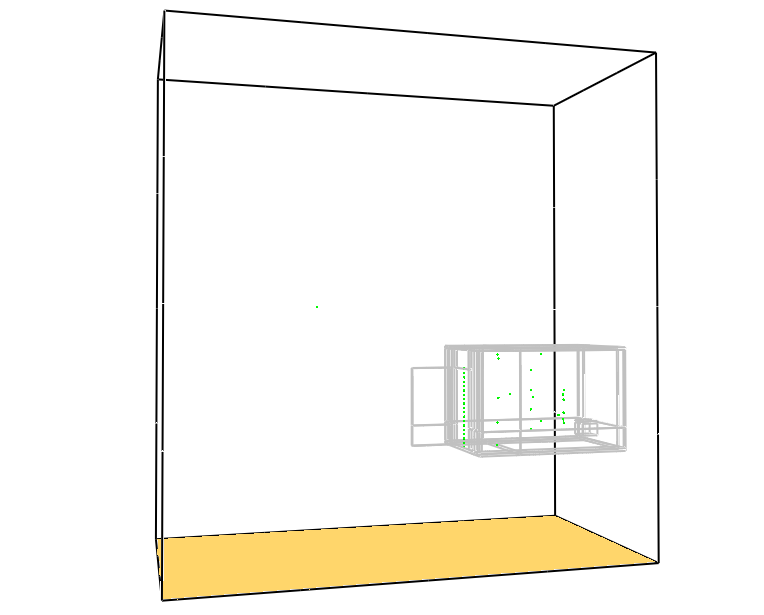
\includegraphics[trim = 50mm 0mm 0mm 0mm, clip,width=0.45\textwidth]{IAFSS_Paper/Figures/NIST_Backdraft_Domain1.png}
    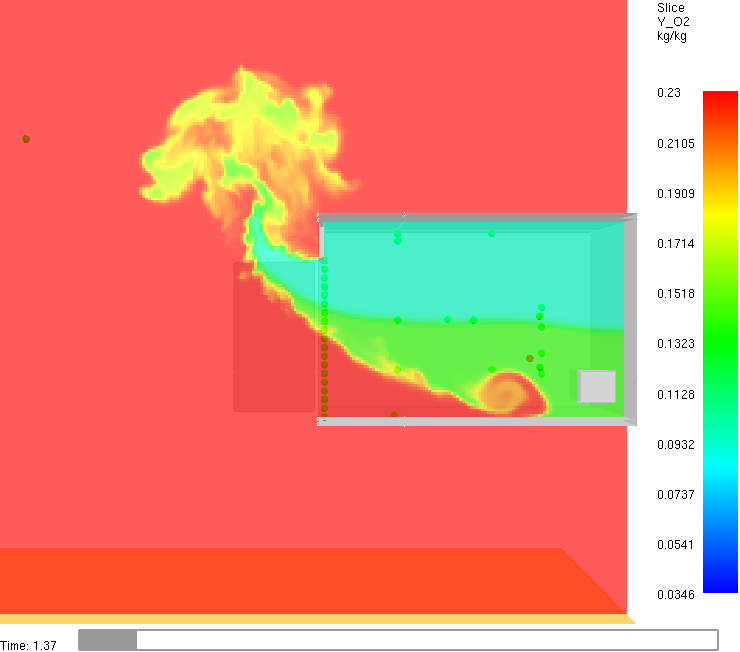
\includegraphics[trim = 0mm 10mm 30mm 0mm, clip,width=0.45\textwidth]{IAFSS_Paper/Figures/NIST_Backdraft_GC1.png}
    \makebox[0.49\textwidth]{(a)}
    \makebox[0.49\textwidth]{(b)} \\
    \caption{Backdraft computational model : (a) Domain and compartment geometry with ignition and data collection devices, door open. (b) Oxygen mass fraction slice (blue to red, 0.04 to 0.23 kg/kg) for representative run showing the incursion of gravity current into the compartment.}
    \label{fig:model_setup}
\end{figure}

A computational model was created to simulate with FDS the backdraft experiments given a representative set of species concentration and temperature initial conditions. FDS6.7.9-1409 was compiled from source using the Intel\textregistered~OneAPI toolchain and used in this work. The Smokeview~\cite{Smokeview_Users_Guide} render of the domain, compartment and ignition/data collection devices can be seen in Figure~\ref{fig:model_setup}a. In all computations, the domain is of size 4.56 m x 2.22 m x 4.84 m in the $x,y,z$ directions, deemed appropriate to capture the combustion region inside and outside the compartment correctly. The domain is divided into 48 meshes. Computations were done using FDS MPI parallel processing capability. The two-step simple chemistry model for fast reactions~\cite{FDS_Users_Guide} was employed to accommodate the different species defined from the experiment (fuel, oxygen, carbon monoxide, carbon dioxide, water vapor, and soot). Default parameters for the chemistry model were used, and soot yields were set to 0.001 kg/kg for methane and 0.024 kg/kg for propane~\cite{SFPE:Tewarson}.
Different grid sizes were evaluated for the range of cases defined by experimental initial conditions: coarse grid $\Delta x=5.7$ cm, medium grid $\Delta x=2.8$ cm, and fine grid $\Delta x=1.4$ cm. Cells were approximately cubed and kept constant in the domain. Also, for two representative backdraft cases shown below, a very fine grid with $\Delta x=0.7$ cm was used to evaluate grid sensitivity. Both the compartment and sand gas burner within were modeled, with the compartment floor at 1 m from the domain floor to mimic the experimental setup. The compartment is defined by adiabatic surfaces, and calculations were done from the door opened condition for 15 s, time sufficient to completely capture the backdraft phenomenon in this problem. Calculations took several minutes to a few days in local clusters at NIST.

As described in the previous section, 10 initial conditions were provided for species volume fractions and temperature in two zones within the compartment separated at a height from the compartment floor of 39.25 cm. Together with the option to define a low or mid-ignition location, 20 different simulations could be performed per grid resolution. Ambient initial conditions were specified outside of the compartment. 
A representative slice of oxygen concentration showing the incursion of the gravity current into the back of the compartment can be seen in figure~\ref{fig:model_setup}b. In this figure, the dot on top of the gravity current front represents the ignition point for the low ignitor configuration. To model the ignition procedure consistently with the re-ignition model, a spark was defined in the corresponding ignitor location (low or mid spark) by placing a \texttt{SPARK} device. The ignition temperature threshold $T_{TH}$ was therefore set to 0 K in the cell containing the device. 

\section{Grid sensitivity and comparisons with experiments}
\label{sec:Grd_sens_exp}

In Table~\ref{tab:grid_sens}, computed average gravity current height at the door $H_{avg}$ and velocity $U_{avg}$, as well as total heat release, $THR$, are given as a function of grid size for two representative backdraft cases. These cases are methane, 25~kW, FFT~=~450~s, and propane, 25~kW, FFT~=~285~s. The fuel load inside the compartment for these was such that a high probability of backdraft was seen in experiments. Both cases exhibited backdraft in calculations. 
The average gravity current height at the door was computed from the average zero of the normal velocity in the door symmetry plane between 0.5~s and 2~s (about the ignition time). Noise was noted on this function given by the vortical structures formed in the shear layer between hot and cold air regions, and this was more pronounced in finer grids, as expected. $U_{avg}$ was computed by dividing the distance from the door to the ignition source by the time taken from door opening to ignition. In the simulations, the ignition time was computed as the time taken for the heat release rate $HRR$ to increase over 0.5kW. In FDS, $THR$ is calculated by integrating equation~\eqref{eq:HRRPUV} in the spatial domain and simulation time interval.
It is seen that these global measures of the fluid evolution and backdraft event tend to converge for these benchmark cases as the grid is refined. Differences in $H_{avg}$ are less than 2\% among fine and very fine grids. Similarly, backdraft measures $U_{avg}$ and $THR$ show differences within 10\%.
%
\begin{table}[]
    \centering
    \begin{tabular}{c|c|c|c|c|c}
    \hline
    Case~[Fuel, Fire Size, FFT]                & Grid         & $\Delta x$~(cm) & $H_{avg}$~(cm) & $U_{avg}$~(m/s) & $THR$~(kJ)   \\ % Tig
    \hline
    Methane, 25~kW, 450~s & coarse   &           5.7 &      43.34        &     0.38      &   2693    \\ % 2.91
    Methane, 25~kW, 450~s & medium   &           2.8 &      44.61        &     0.49      &   2665    \\ % 2.25
    Methane, 25~kW, 450~s & fine     &           1.4 &      44.79        &     0.47      &   3580    \\ % 2.35
    Methane, 25~kW, 450~s & very fine &           0.7 &      44.51        &     0.47      &  \textcolor{red}{3619}         \\ % 2.32
    \hline
    Propane, 25~kW, 285~s & coarse   &           5.7 &      43.61         &    0.39       &   2357   \\ % 2.82
    Propane, 25~kW, 285~s & medium   &           2.8 &      44.41         &    0.51       &   2534   \\ % 2.14
    Propane, 25~kW, 285~s & fine     &           1.4 &      44.41         &    0.50       &   2716   \\ % 2.22
    Propane, 25~kW, 285~s & very fine &           0.7 &      44.93         &    0.55       &   2780   \\ % 1.97
    \hline
    \end{tabular}
    \caption{Grid sensitivity of two representative backdraft cases using methane and propane as fuels and low ignitor. Cases run in FDS LES mode, \texttt{EXTINCTION\_2} extinction model and $T_{TH}=300^o$C.}
    \label{tab:grid_sens}
\end{table}

\textcolor{red}{For reference, the total heat release measured in experiments for the methane, 25~kW, FFT~=~450s case was 3470~kJ $\pm$ 520~kJ, and for the propane, 25~kW, FFT~=~285~s case, was 2886~kJ $\pm$ 370~kJ. The dominating factor in the total heat release uncertainty attributes to the Type A evaluation of uncertainty, specifically the variance between repeated runs. The average total heat release measurements differ by about 30\% and 6\% with respect to the corresponding coarse and fine grid calculations. We note that fine grid calculations are within the uncertainty computed for these experimental ensemble averages}. Also, the average gravity current height at the door estimated from video analysis of the Propane, 25~kW, FFT~=~285~s case is 44.7~cm, differing about 2.5~\% and 1~\% with respect to coarse and fine grid estimates. Experimental $U_{obs}$ computed from video analysis of time for ignition is 0.7~m/s and 0.5~m/s, respectively, in agreement with fine grid computation results (0.47~m/s and 0.50~m/s) and analytical estimations~\cite{fleischmann1993backdraft}. Gravity current estimated velocity values $U_{est}$ are 0.48~m/s for the methane, 25~kW, FFT~=~450~s case, and 0.50~m/s for the propane, 25~kW, FFT~=~285~s case. 

Experiment pictures and simulation renders of the fireball exit for the Propane, 25~kW, FFT~=~285s case are shown in Figure~\ref{fig:prop_fire}. In the simulation, Smokeview rendered pixels are colored where the heat release rate per unit volume is greater than $200$~kW.m$^{-3}$ and the temperature is higher than $600^o$C. Experiment and simulation quantities are not the same in this figure, but they provide insight into how the deflagration behaves in both cases. It is seen that the horizontal ejection of the deflagration is slightly weaker in the simulation, consistent with a slower evolution within the compartment. The time taken from door opening to fireball exit was estimated to be 2.66~s~$\pm$~0.7, whereas this quantity in the fine grid simulation was 3.9~s. 
This result was seen using both extinction models, albeit less pronounced for \texttt{EXTINCTION\_1} (3.1~s), and also in 
methane simulations. The burning region close to the compartment's floor, as seen in calculations of Figure~\ref{fig:prop_fire}, is consistent with higher density and concentration of propane at door opening time.

%
\begin{figure}[tb]
    \centering
    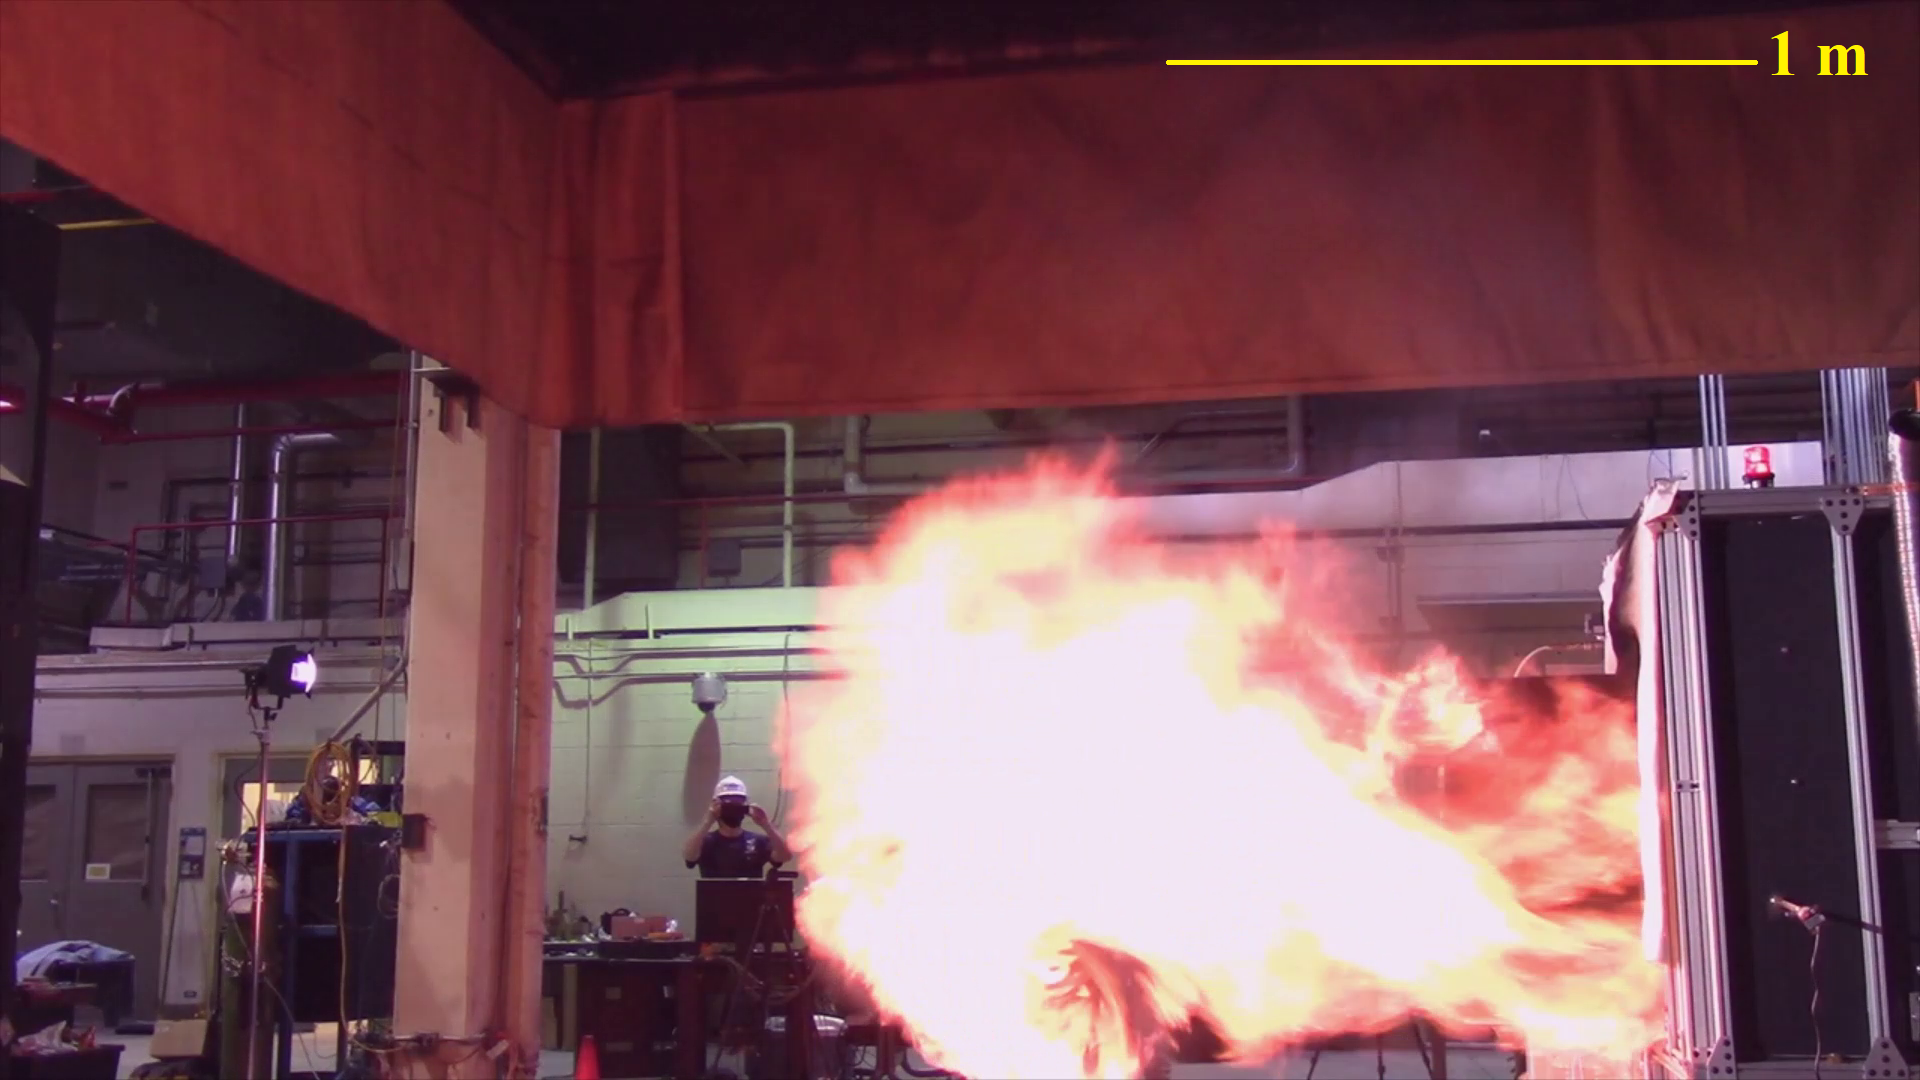
\includegraphics[trim = 0mm 0mm 0mm 0mm, clip,width=0.48\textwidth]{IAFSS_Paper/Figures/246 vlcsnap-2023-01-30-22h18m26s991.png}
    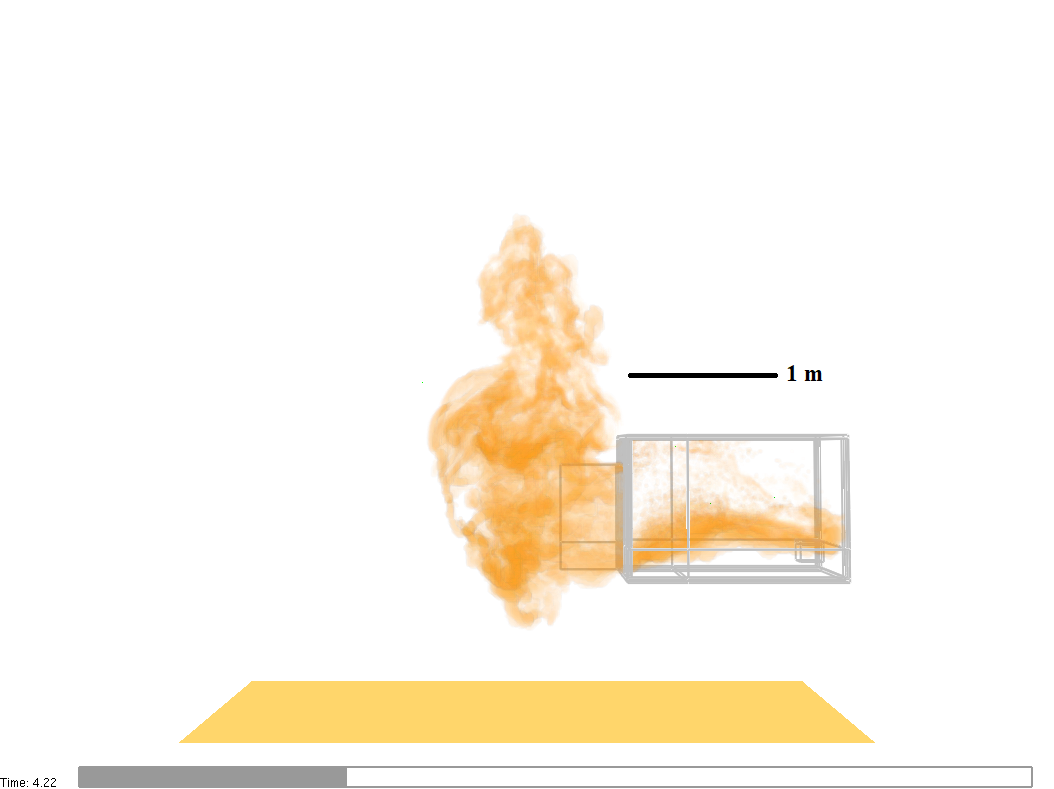
\includegraphics[trim = 50mm 50mm 60mm 80mm, clip,width=0.48\textwidth]{IAFSS_Paper/Figures/NIST_Backdraft_Propane_25kW_285s_low_EXT2_HRRPUV_4p22s.png}
    \makebox[0.49\textwidth]{(a)}
    \makebox[0.49\textwidth]{(b)} \\
    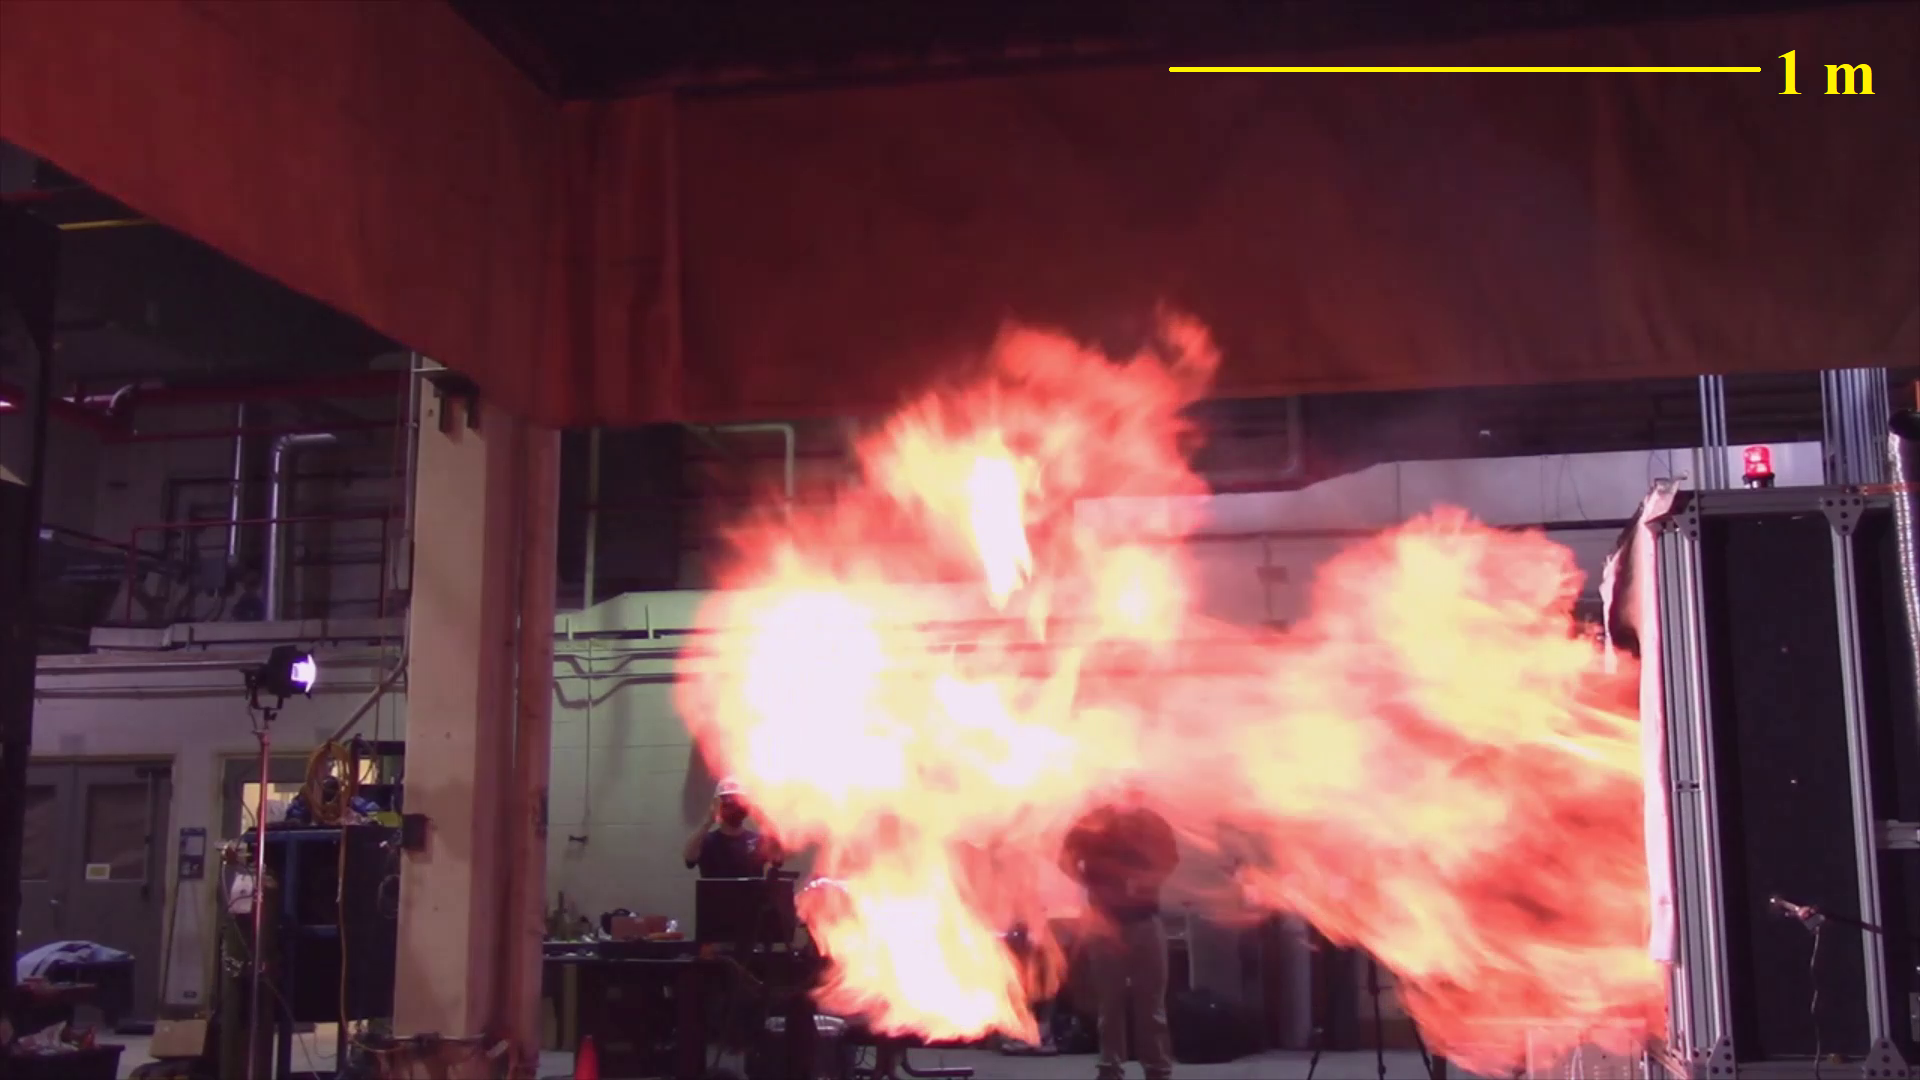
\includegraphics[trim = 0mm 0mm 0mm 0mm, clip,width=0.48\textwidth]{IAFSS_Paper/Figures/246 vlcsnap-2023-01-30-22h18m40s863.png}
    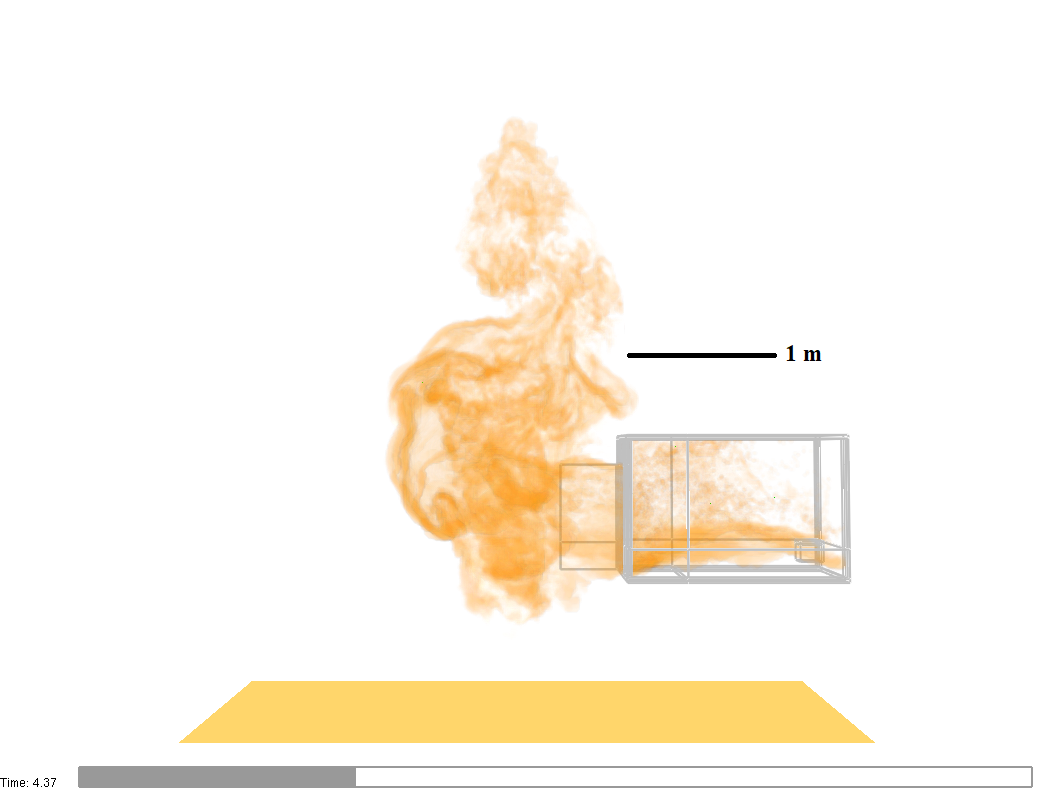
\includegraphics[trim = 50mm 50mm 60mm 80mm, clip,width=0.48\textwidth]{IAFSS_Paper/Figures/NIST_Backdraft_Propane_25kW_285s_low_EXT2_HRRPUV_4p37s.png}
    \makebox[0.49\textwidth]{(c)}
    \makebox[0.49\textwidth]{(d)}    
    \caption{Backdraft exit deflagration from the door for propane, 25~kW, FFT~=~285s case. (a) Experiment photograph at $t~=~2.73$ from the door opening, (b) Smokeview HRRPUV render for fine grid simulation $t=4.22$~s, (c) Experiment $t=2.90$, and (d) Simulation $t=4.37$~s.}
    \label{fig:prop_fire}
\end{figure}
%

Most importantly, in the calculations of Table~\ref{tab:grid_sens}, the ignition threshold $T_{TH}$ was set to $300^o$C. As shown in the next section, the number assigned to this parameter is critically important to obtain deflagration on numerical simulations of backdraft with fast mixing-controlled chemical reactions.

\section{Effect of ignition threshold}
\label{sec:ign_thr}

%
\begin{figure}[tb]
    \centering
    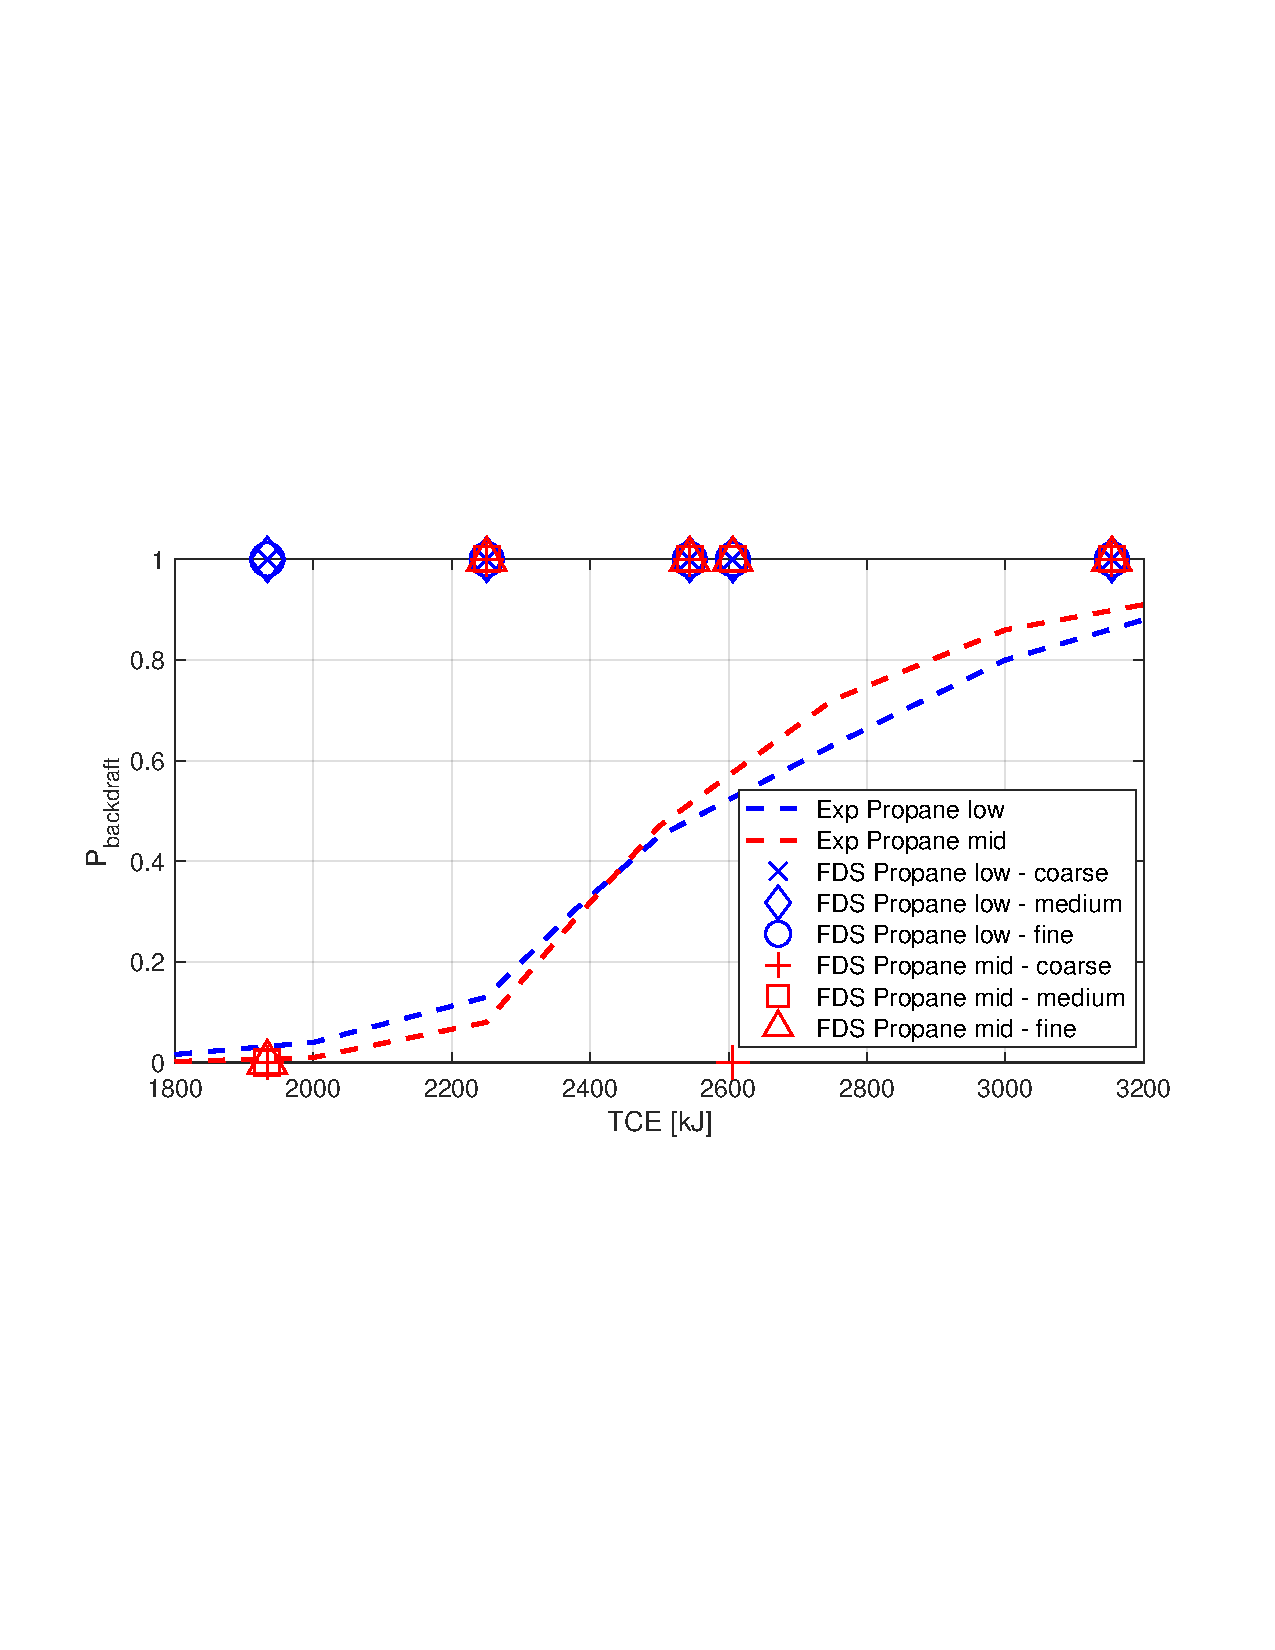
\includegraphics[trim = 14.5mm 85mm 17mm 80mm, clip,width=0.505\textwidth]{IAFSS_Paper/Figures/PbvsTCE_Cign_LES_Extinction_2_TTH300_Propaneb.pdf}
    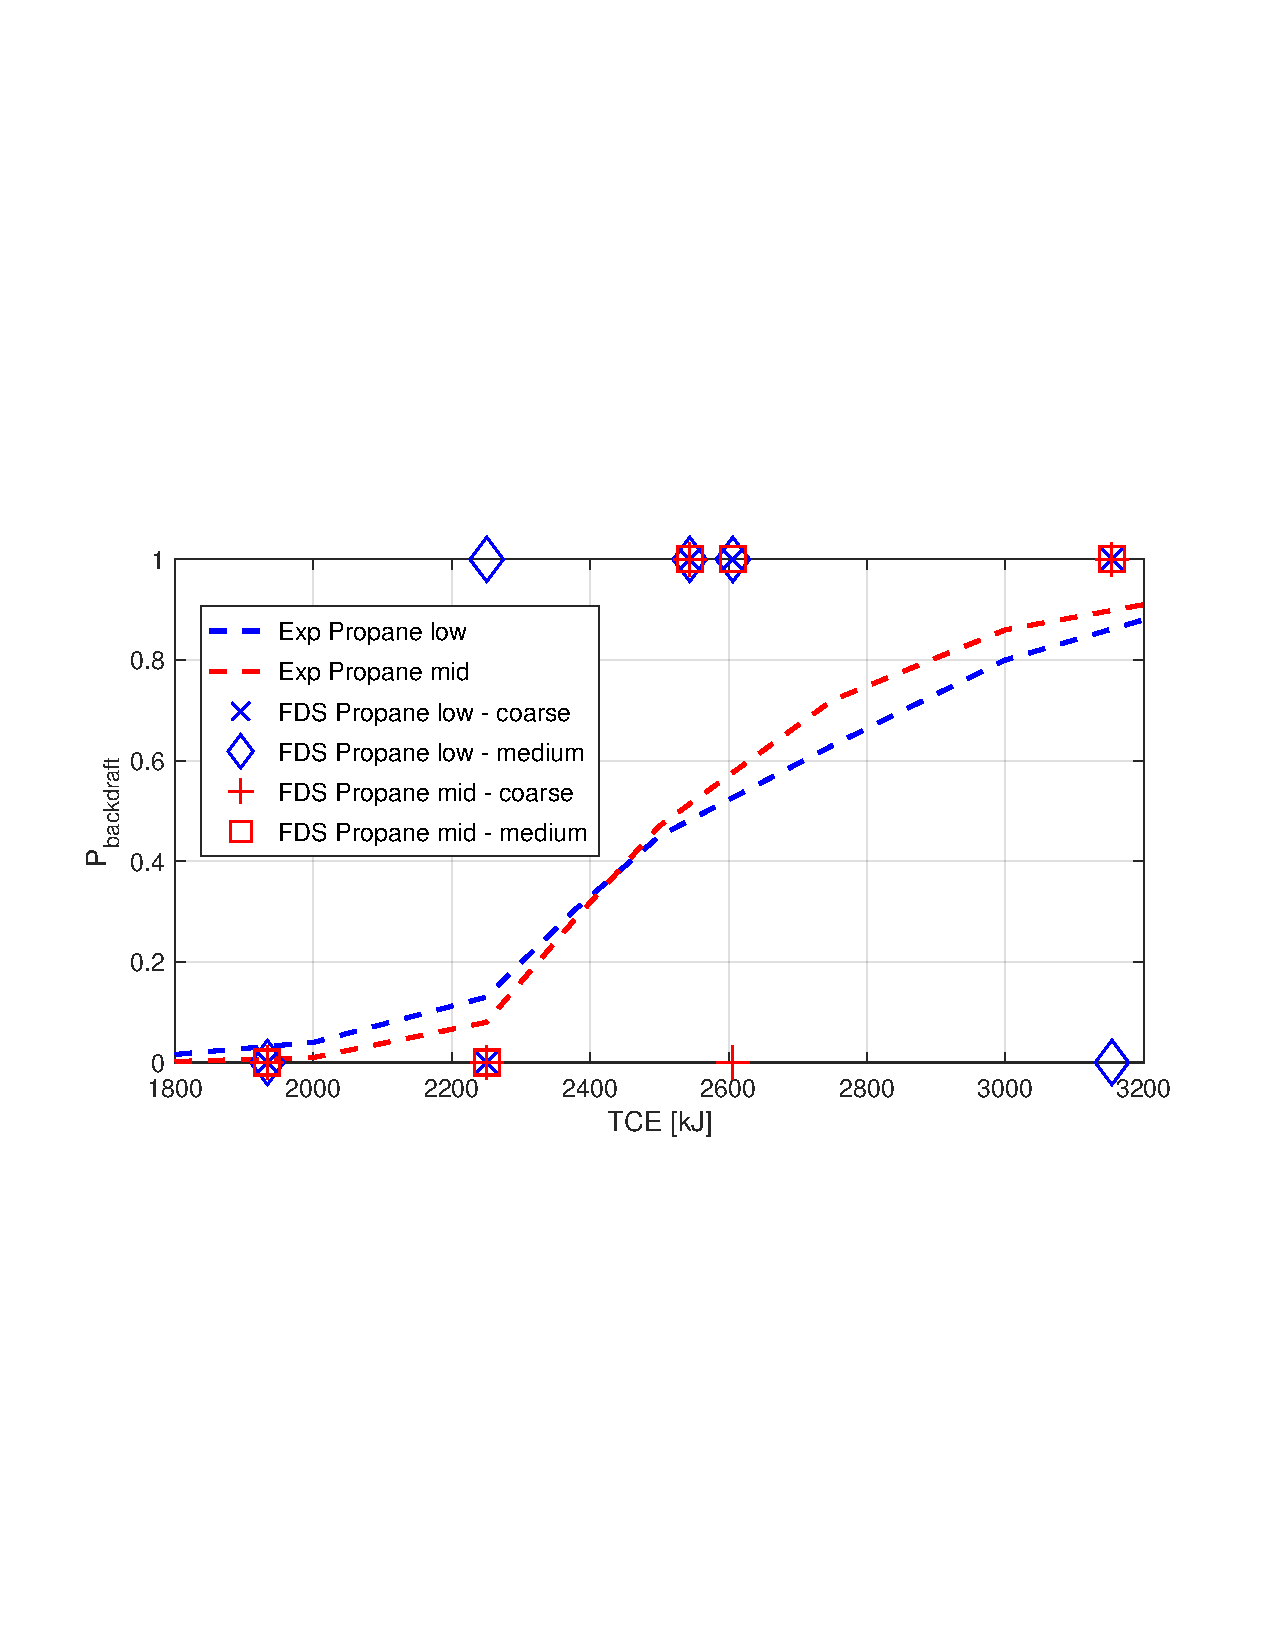
\includegraphics[trim = 22mm 85mm 17mm 80mm, clip,width=0.485\textwidth]{IAFSS_Paper/Figures/PbvsTCE_Cign_LES_Extinction_2_TTH325_Propaneb.pdf}
    \makebox[0.50\textwidth]{(a)}
    \makebox[0.48\textwidth]{(b)} \\
    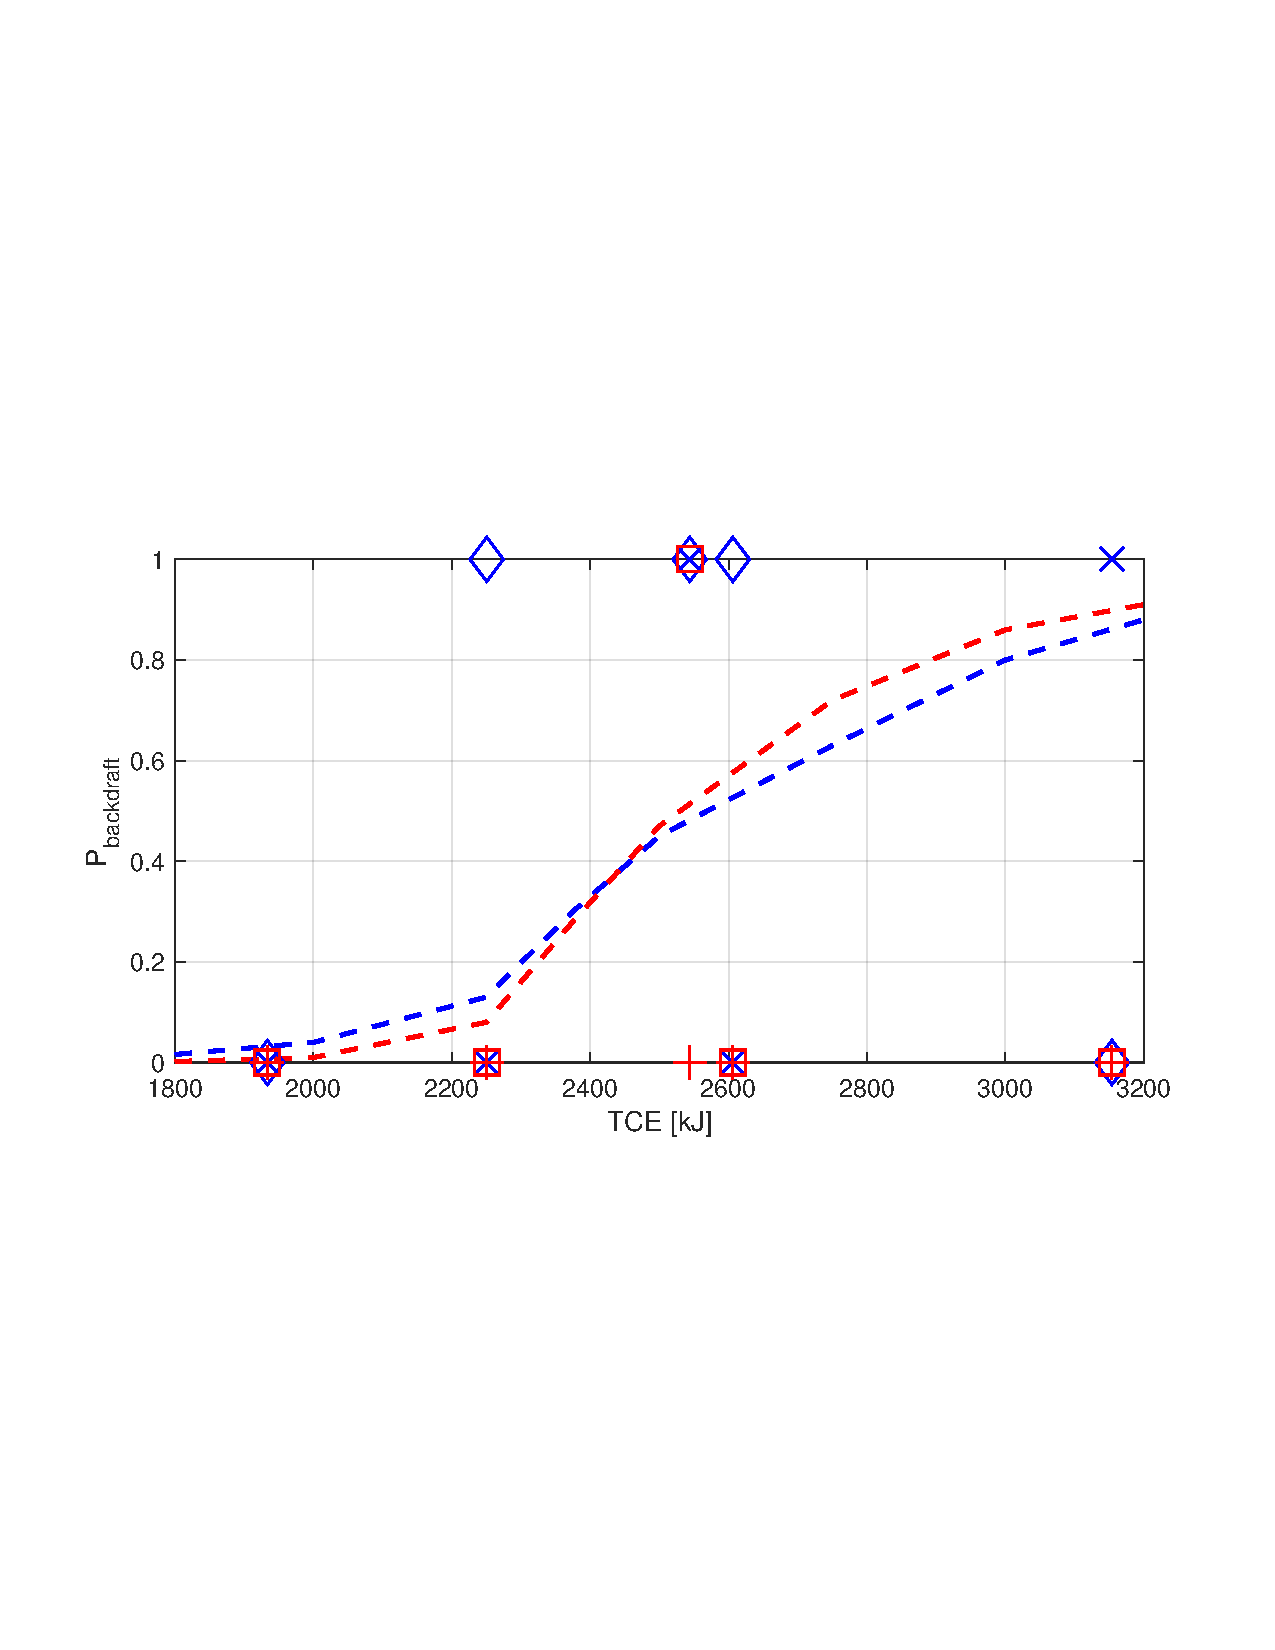
\includegraphics[trim = 14.5mm 85mm 17mm 80mm, clip,width=0.505\textwidth]{IAFSS_Paper/Figures/PbvsTCE_Cign_LES_Extinction_2_TTH350_Propaneb.pdf}
    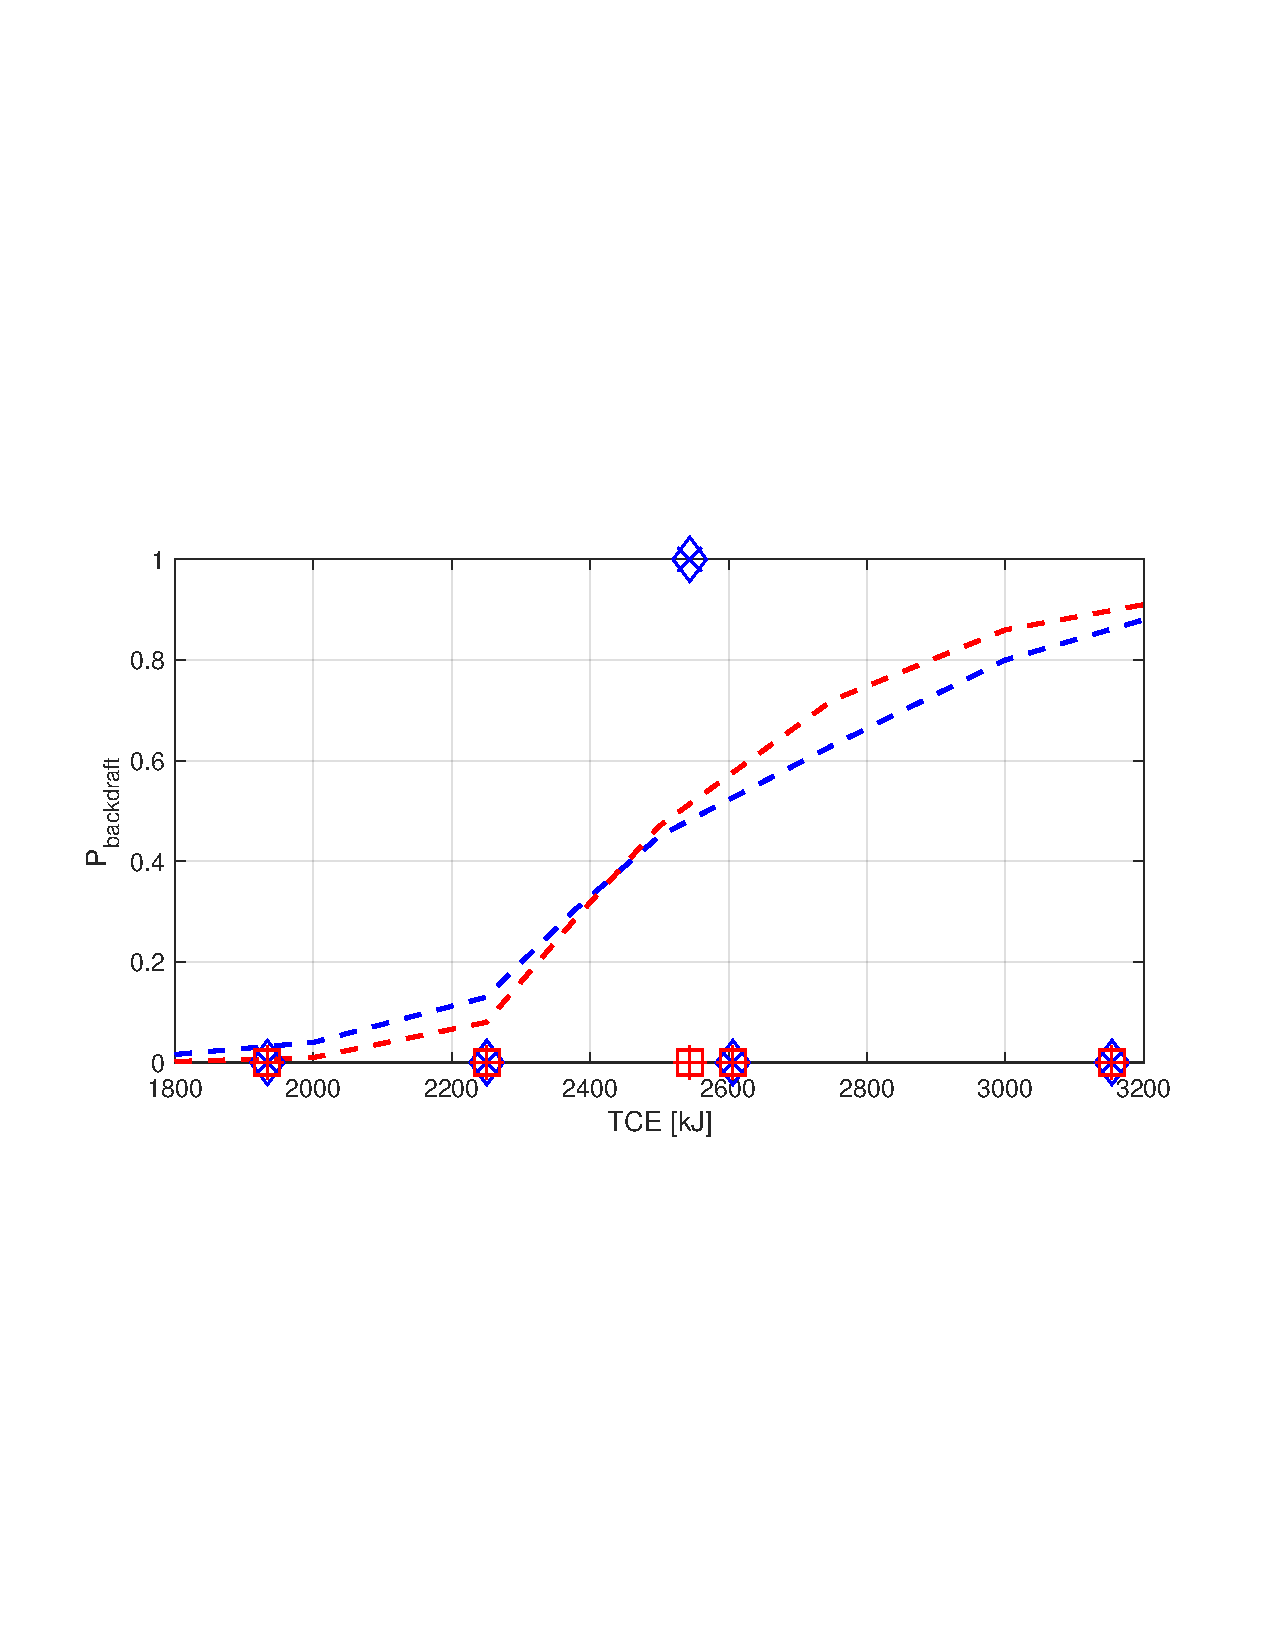
\includegraphics[trim = 22mm 85mm 17mm 80mm, clip,width=0.485\textwidth]{IAFSS_Paper/Figures/PbvsTCE_Cign_LES_Extinction_2_TTH400_Propaneb.pdf}
    \makebox[0.50\textwidth]{(c)}
    \makebox[0.48\textwidth]{(d)}    
    \caption{Simulated Backdraft events as a function of total fuel chemical energy $TCE$ for propane. (a) Ignition model $T_{TH}=300^o$C, (b) $T_{TH}=325^o$C, (c) $T_{TH}=350^o$C, and (d) $T_{TH}=400^o$C. }
    \label{fig:Pb_ign}
\end{figure}
%
The re-ignition model $T_{TH}$ primarily affects backdraft simulations with fast chemistry. To get an estimate for defining if the backdraft event happened in simulations, a test was devised comparing the total heat release $THR$ and total heat release outside of the compartment $THR_{EXT}$ with respect to the initial total chemical energy, $TCE$, of the fuel within the compartment. This last value is computed as $TCE=M_F \; \Delta H_F^{\rm{o}}$, where $M_F$ is the initial mass of fuel in the compartment, and $\Delta H_F^{\rm{o}}$ is the fuel's heat of combustion obtained from Ref.~\cite{Hurley2016}. Therefore, $TCE$ is the maximum amount of thermal energy that can be produced by combustion. Backdraft is assumed to have happened if $THR>C_1 \; TCE$ and $THR_{EXT}>C_2 \; THR$. The constants $C_1$ and $C_2$ were set to 0.3, a value found to be sufficient to determine the deflagrations seen in the simulations. 

It was noted initially that using the default fuel auto-ignition temperature for $T_{TH}$ would lead to having no deflagration for any of the 20 initial condition sets, irrespective of the grid refinement used. AITs in FDS are taken from reference~\cite{SFPE:Beyler} and are for methane and propane $540^o$C and $450^o$C, respectively. 
\textcolor{red}{In Figure~\ref{fig:Pb_ign}, plots of backdraft events as a function of $TCE$ for propane and different values of $T_{TH}=300,325,350,400^o$C are shown, for both "low" and "mid" ignitor positions. Superimposed are the backdraft probability, $P_{Backdraft}$, curves computed from the experiment, also as a function of the compartment fuel chemical energy load. It is emphasized that the results of simulations are \textit{deterministic}. Therefore, in order to visualize their progression, "backdraft happened" in the simulations is assigned a value $P_{Backdraft}=1$ in these plots, and "backdraft didn't happen" is given a $P_{Backdraft}=0$.} In Figure~\ref{fig:Pb_ign}a,  $T_{TH}=300^o$C, fine grid results are also shown. Generally, the outcomes were not different between medium and fine refinement grids.

It is also observed that the backdraft outcomes are highly dependent on the temperature threshold of the FDS default re-ignition model. Within a small range of $100^o$C, outcomes range from "deflagration happened" being strongly over-predicted, to practically "no deflagration" simulated. This result is independent of the fuel load in the compartment. A value of $T_{TH}=325^o$C gives the best approximation to experiment-derived backdraft probability curves. 
Ideally, a good representative value of $T_{TH}$ could be found, although it is unclear how that would have to be modified in different scenarios and for other fuels. This poses a great challenge for simulating these transient events using fast chemistry. We also note that analogous behavior was seen using the temperature controlled \texttt{EXTINCTION\_1} method.
Similar trends were seen for methane, albeit transition was found to happen at a slightly lower temperature threshold for the ignition model, and more event variability with $TCE$ was seen. 

\section{Effect of ignition procedure}
\label{sec:ign_proc}

%
\begin{figure}[h]
    \centering
    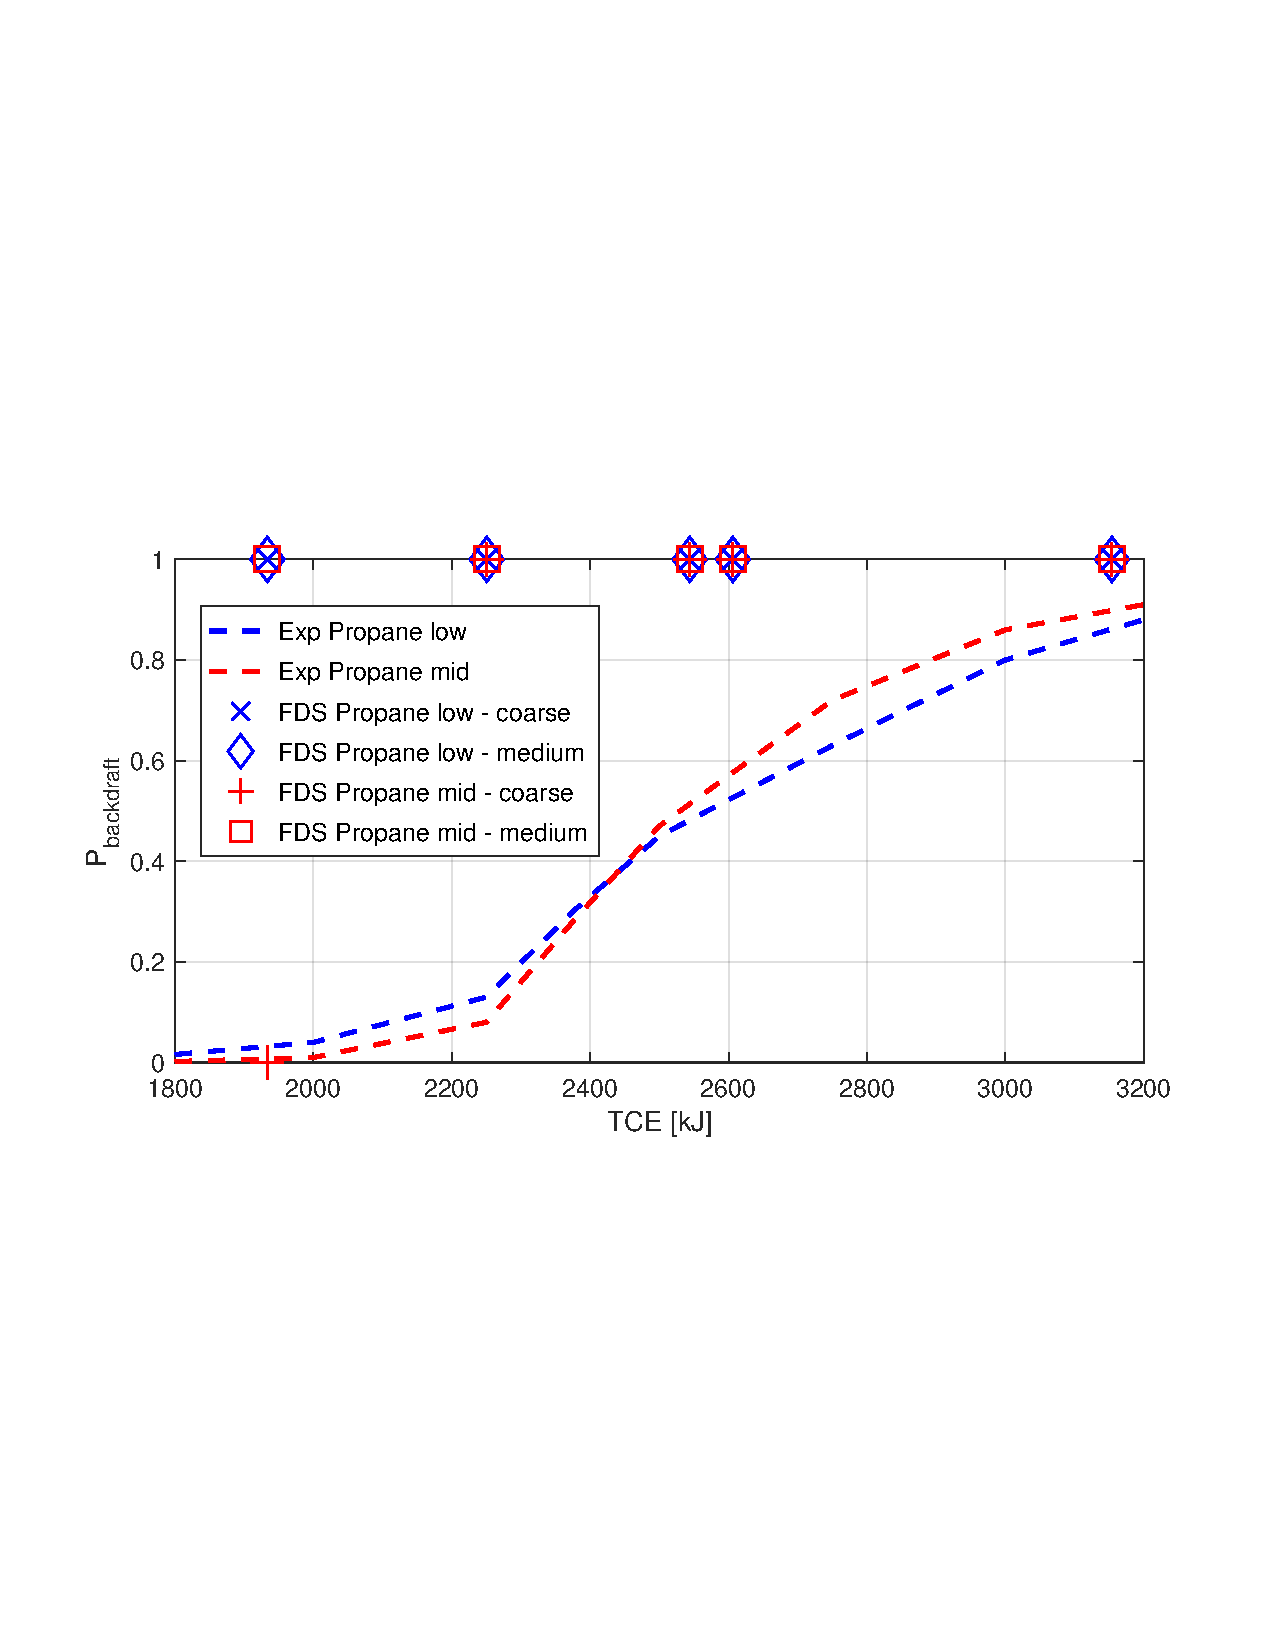
\includegraphics[trim = 14.5mm 85mm 17mm 80mm, clip,width=0.505\textwidth]{IAFSS_Paper/Figures/PbvsTCE_Cign_LES_Extinction_2_TTH300_LGIGN_Propaneb.pdf}
    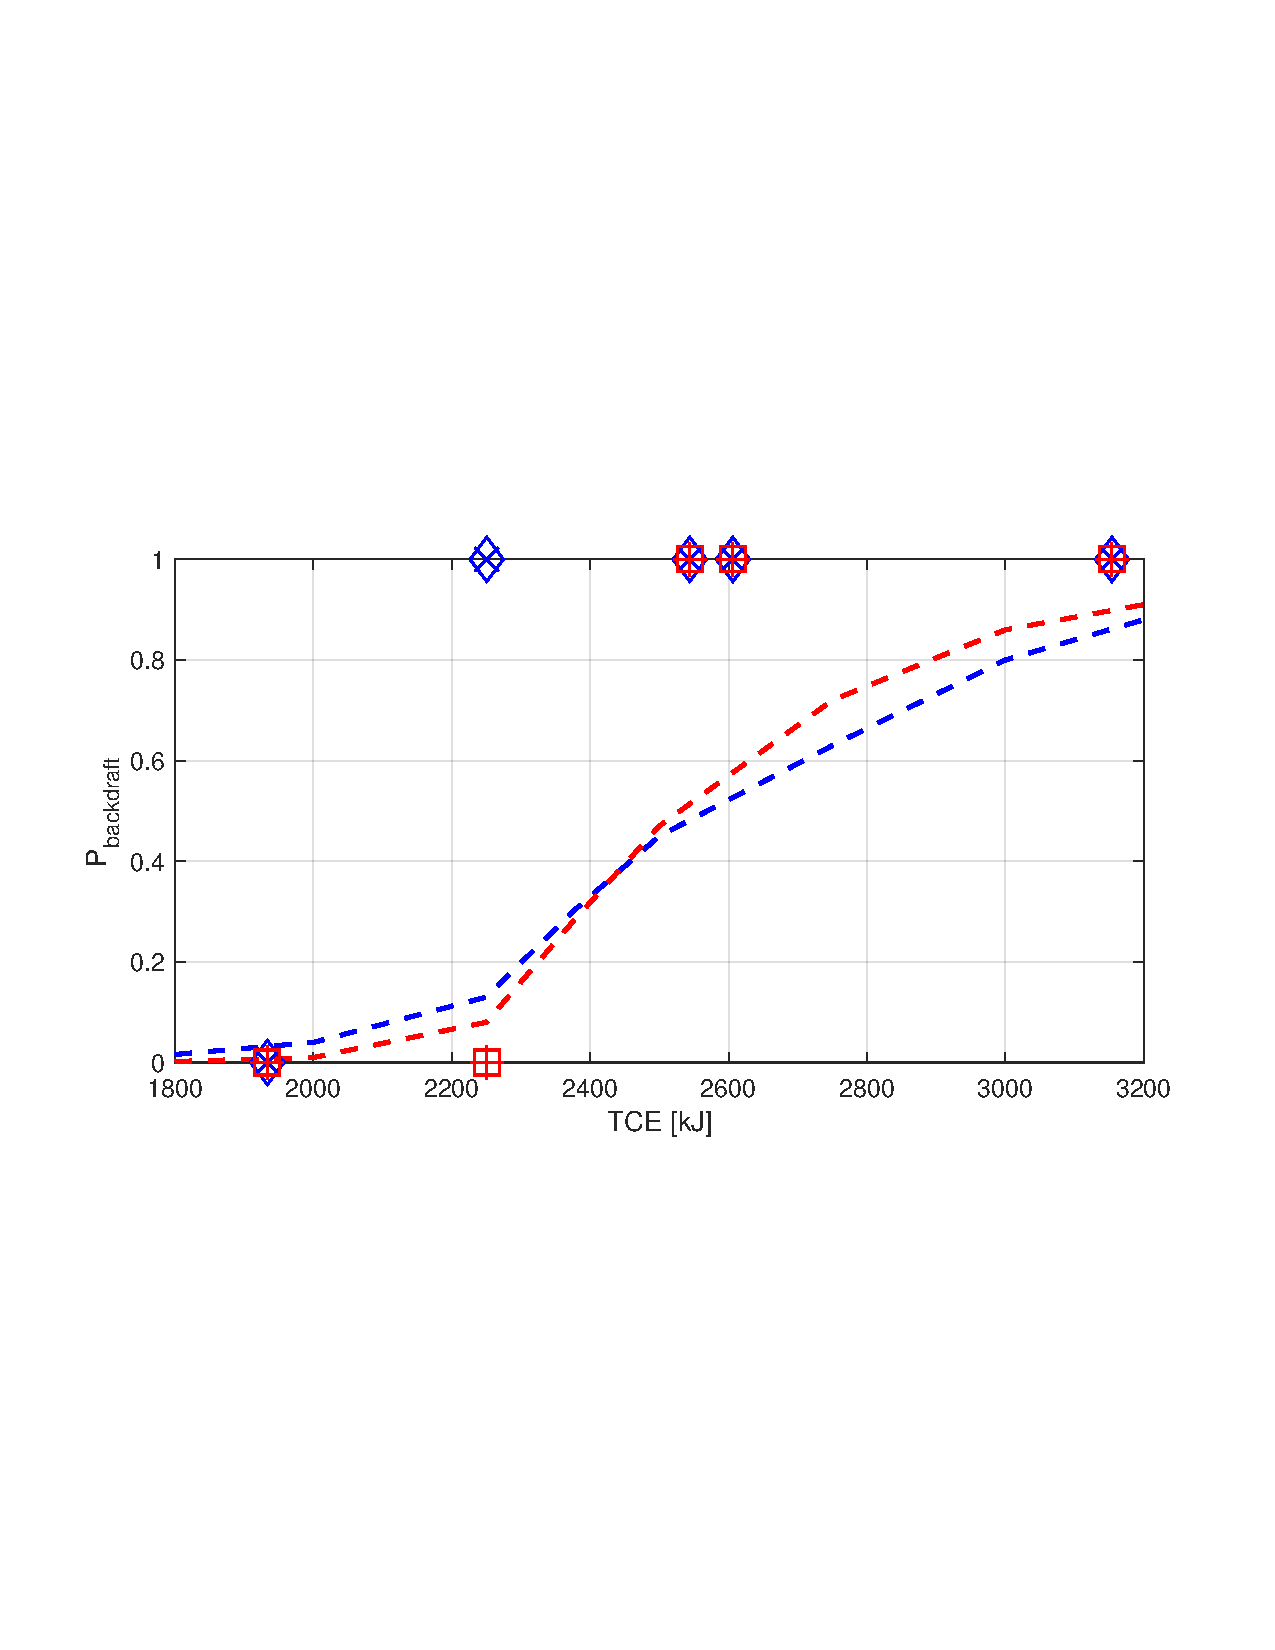
\includegraphics[trim = 22mm 85mm 17mm 80mm, clip,width=0.485\textwidth]{IAFSS_Paper/Figures/PbvsTCE_Cign_LES_Extinction_2_TTH350_LGIGN_Propaneb.pdf}
    \makebox[0.50\textwidth]{(a)}
    \makebox[0.48\textwidth]{(b)} \\
    \caption{Simulated Backdraft events as a function of total fuel chemical energy $TCE$ for propane and 8 spark grid ignitor. (a) Ignition model $T_{TH}=300^o$C, (b) $T_{TH}=350^o$C. }
    \label{fig:Pb_ignproc}
\end{figure}
%
To test the effect of the ignition procedure in backdraft outcomes, a grid of 8 \texttt{SPARK} devices was defined in a horizontal plane area of 2 cm by 6 cm located near the experiments' ignition spark location. This resulted in a larger mesh volume that would undergo combustion in the ignitor region for each grid resolution, as the corresponding computational cells were assigned $T_{TH}=0$~K. For comparison, in Figure~\ref{fig:Pb_ignproc}, similar plots to Figure~\ref{fig:Pb_ign} are shown for this larger spark ignitor.

In terms of backdraft events, the effect of having a larger ignition volume is akin to using a slightly lower $T_{TH}$ in this problem. A larger ignitor volume where air and fuel can mix and react potentially produces higher heat release and temperatures in computational cells surrounding the ignition region. This leads to a larger chance of prompting deflagration. Similar issues have been found when modeling piloted ignition of burners as observed in Ref.~\cite{White:2017}. Although this behavior is expected, it also points to the difficulty of modeling the complex thermo-chemical process of fuel ignition by a spark when using simplified mixing-controlled combustion.

\section{Conclusions}
\label{sec:concl}

In this work, a wealth of experimental data was leveraged to define initial conditions and validation information, which can be used to assess the capability of fire models in simulating backdraft phenomena. Initial condition text data can be obtained by contacting the authors. A model for said experiments was developed within the FDS framework and used to test the simulation software with standard mixing-controlled fast chemical reactions.

\textcolor{red}{Comparison with experiments of global backdraft quantities showed good agreement in relatively fine grids and select high fuel load cases. Nevertheless, it was seen that backdraft simulation presents a great challenge for fast chemistry combustion models used in realistic engineering applications. In particular, simple ignition models based on a temperature threshold require tuning this parameter. It was noted that variations of $50^o$C on this parameter could significantly change backdraft outcomes across various grids, ignition sources, and initial conditions.} Ideally, a variation of the re-ignition model that is not as sensitive to a hand-picked temperature parameter would be available. An option being considered by this group is the use of a test temperature that is not only the mean cell temperature but also contains a subgrid component. 

On the other hand, it was shown that the ignition procedure based on dropping the temperature threshold at the ignition source location also greatly influences the backdraft simulation outcome. It is unclear how the ignition volume should be defined for backdraft triggered by point sources like sparks, and more study is required on this topic. \textcolor{red}{Further, in these calculations uniform composition and temperature conditions in two zones were used from experiment sensor averages. The effect of this simplification in the results should be tested. One possible way is to actually simulate the fuel loading process in the compartment up to door opening. Another option is to add stochastic disturbances of initial composition fields to assess their effect in backdraft outcomes.} 

\textcolor{red}{Finally, the experiments modeled in this work involved simple hydrocarbon gases, with known chemical and thermal properties. In real fires, gaseous fuels are the product of complex pyrolysis processes and therefore backdraft outcomes are expected to be heavily influenced by their combustion characteristics. Although not touched upon, experiments similar to the ones described section~\ref{sec_exp_meth} were also performed using wood-cribs as fuel. Their modeling and analysis is left for a future effort.} 

%\section*{References}
\bibliographystyle{elsarticle-num}
\bibliography{References}
	
\newpage %The figure captions section must be on a separate page.
\section*{Figure captions}
Figure~\ref{fig:Backdraft_experimental_setup}. Schematic of the $2/5^{\rm{th}}$ scale compartment used in backdraft experiments

Figure~\ref{fig:model_setup}. Backdraft computational model : (a) Domain and compartment geometry with ignition and data collection devices, door open. (b) Oxygen mass fraction slice (blue to red, 0.04 to 0.23 kg/kg) for representative run showing the incursion of gravity current into the compartment.

Figure~\ref{fig:prop_fire}.Backdraft exit deflagration from the door for propane, 25~kW, FFT~=~285s case. (a) Experiment photograph at $t~=~2.73$ from the door opening, (b) Smokeview HRRPUV render for fine grid simulation $t=4.22$~s, (c) Experiment $t=2.90$, and (d) Simulation $t=4.37$~s.

Figure~\ref{fig:Pb_ign}. Simulated Backdraft events as a function of total fuel chemical energy $TCE$ for propane. (a) Ignition model $T_{TH}=300^o$C, (b) $T_{TH}=325^o$C, (c) $T_{TH}=350^o$C, and (d) $T_{TH}=400^o$C.

Figure~\ref{fig:Pb_ignproc}. Simulated Backdraft events as a function of total fuel chemical energy $TCE$ for propane and 8 spark grid ignitor. (a) Ignition model $T_{TH}=300^o$C, (b) $T_{TH}=350^o$C.



\end{flushleft}
\end{document}